% SPDX-FileCopyrightText: 2023 SAP SE
%
% SPDX-License-Identifier: Apache-2.0
%
% This file is part of FEDEM - https://openfedem.org

%%%%%%%%%%%%%%%%%%%%%%%%%%%%%%%%%%%%%%%%%%%%%%%%%%%%%%%%%%%%%%%%%%%%%%%%%%%%%%%%
%
% FEDEM User Guide.
%
%%%%%%%%%%%%%%%%%%%%%%%%%%%%%%%%%%%%%%%%%%%%%%%%%%%%%%%%%%%%%%%%%%%%%%%%%%%%%%%%

\Chapter{Introduction to Fedem}{introduction-to-fedem}

Welcome to Fedem! This chapter gives an overview of the Fedem software and its
technological foundation. It explains what a Fedem model is, and outlines the
different program modules.

Sections in this chapter address the following topics:

\begin{itemize}
\item
  \protect\hyperlink{what-is-fedem}
                    {What is Fedem?}
\item
  \protect\hyperlink{nonlinear-structural-dynamics}
                    {Nonlinear structural dynamics}
\item
  \protect\hyperlink{what-is-a-fedem-model}
                    {What is a Fedem model?}
\item
  \protect\hyperlink{control-systems-in-mechanical-analysis}
                    {Control systems in mechanical analysis}
\item
  \protect\hyperlink{using-fe-models}
                    {Using FE models}
\item
  \protect\hyperlink{fedem-solver-modules}
                    {Fedem solver modules}
\end{itemize}

\clearpage


%%%%%%%%%%%%%%%%%%%%%%%%%%%%%%%%%%%%%%%%%%%%%%%%%%%%%%%%%%%%%%%%%%%%%%%%%%%%%%%%
\Section{What is Fedem?}{what-is-fedem}

Fedem, an acronym for \textbf{F}inite \textbf{E}lement \textbf{D}ynamics
in \textbf{E}lastic \textbf{M}echanisms provides both a technology
platform and an engineering framework for
virtual testing of complex mechanical assemblies. It provides a
complete set of features to create, solve and post-process a model
in a 3D graphical environment. Dynamics results in the form of
curves and animations are available during and after model solution.
Combined with the fast and numerically stable Fedem solver,
the user interface facilitates an engineering process with
shortened turnaround times and quick access to simulation results
for a clearer understanding of the physical behavior of the model.
Fedem also provides intuitive and high-performing post-processing
capabilities, including full stress analysis, eigenmode solutions,
strain gage solutions and fatigue analysis for selected time steps.

\medskip\noindent
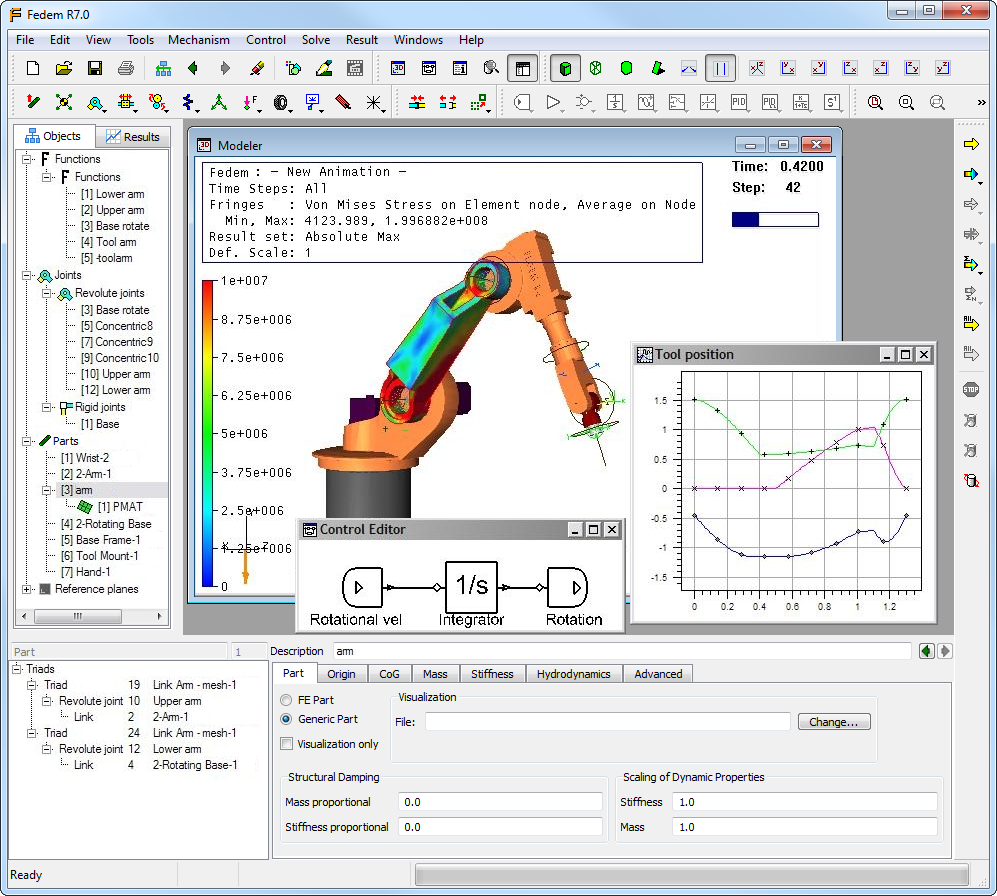
\includegraphics[width=\textwidth]{Figures/1-introduction}


%%%%%%%%%%%%%%%%%%%%%%%%%%%%%%%%%%%%%%%%%%%%%%%%%%%%%%%%%%%%%%%%%%%%%%%%%%%%%%%%
\Section{Nonlinear structural dynamics}{nonlinear-structural-dynamics}

In multibody applications such as suspension systems, axle systems,
car bodies, satellite appendages, industrial manipulators, medical
equipment, high-speed mechatronic systems and so on, some of the
mechanism components can be flexible and can experience large
elastic deflections and coupling effects. To ensure sufficient
accuracy, the simulation solver must account for the mutual
dependencies between dynamic properties at the system level and
structural flexibility at the component level. These requirements
can be efficiently satisfied through a nonlinear structural
dynamics approach.

In Fedem, a nonlinear structural dynamics approach is utilized
in order to simultaneously solve structural deformations and
3D motion dynamics in the time domain. The mechanical assembly
to be simulated is comprised of structural Parts, each
represented by a linear elastic finite element (FE) model
or a simplified stiffness description, and coupled together
with linear or nonlinear joints. After a model reduction of
each FE part based on a dynamic superelement formulation, the
system equations are assembled and solved with respect to FE
degrees of freedom (DOFs), allowing large translations and
rotation due to a co-rotated theory.


%%%%%%%%%%%%%%%%%%%%%%%%%%%%%%%%%%%%%%%%%%%%%%%%%%%%%%%%%%%%%%%%%%%%%%%%%%%%%%%%
\Section{Control systems in mechanical analysis}{control-systems-in-mechanical-analysis}

A mechanical system is often in a control loop including sensors
measuring states in the mechanism, compensators representing control
algorithms, and servo, hydraulic, or electrical actuators that
generate the energy to drive the mechanism. These control modules
and the mechanism must be integrated simultaneously in order to
ensure sufficient accuracy of the simulation results.

To model your control systems, Fedem provides the Control Editor
modeling environment, which combines the Fedem look-and-feel with graphical
modeling tools similar to those of MATLAB\Registered/Simulink\Registered.
These modeling tools are crucial when creating models of
mechanical systems such as robots, milling machines,
and space mechanisms.
See \refSection{touring-the-interface}{Touring the interface}
and \refChapter{control-system-modeling}{Control System Modeling}
for more information about the Control Editor.

\clearpage


%%%%%%%%%%%%%%%%%%%%%%%%%%%%%%%%%%%%%%%%%%%%%%%%%%%%%%%%%%%%%%%%%%%%%%%%%%%%%%%%
\Section{What is a Fedem model?}{what-is-a-fedem-model}

A Fedem model is a virtual test model designed by you to
simulate your mechanical systems. The virtual test model
is an assembly of individual parts. The mechanical properties
of the parts can be represented by either an FE model or a
simplified stiffness description. You connect parts, virtual
joints, springs, and other elements to create an accurate
virtual test model of a movable mechanical system or mechanism.

In order to minimize the time needed to calculate and simulate
mechanisms, a model reduction process is used to reduce the FE
models of the mechanism into superelements with external nodes.
These external nodes are defined at FE nodes that serve as
connections between the various model entities in the assembly.

Once constructed, a Fedem model retains the FE characteristics
of its component parts, and can therefore be treated as a
geometrically nonlinear FE model. The mechanism is then allowed
to experience large translations, rotations, and nonlinear,
behavior-dependent loads in the simulation of its dynamic motion.
Functions, measured time history input data and control
systems can be used to model virtual test events by controlling
loads, motion, spring lengths, etc.
The Fedem solvers can then calculate the motion kinematics,
dynamics, structural flexibility, stresses, strains, and
varying loads in one consistent model.


%%%%%%%%%%%%%%%%%%%%%%%%%%%%%%%%%%%%%%%%%%%%%%%%%%%%%%%%%%%%%%%%%%%%%%%%%%%%%%%%
\Section{Using FE models}{using-fe-models}

Fedem imports FE models created in external systems by interfacing with
the MSC.Nastran\Registered Bulk Data File (\File{.bdf} and \File{.nas}) format
(see \refSection{creating-parts-by-file-import}{Creating parts by file import}).
Many FE modeling systems (including I-DEAS\Registered, Pro/ENGINEER\Registered,
Altair\Registered HyperMesh\Registered, NEiWorks/NEiFusion and
MSC/Patran\Registered) can export data to the Bulk Data File format,
enabling you to use your favorite FE modeling program with Fedem.
Fedem can also import models defined in the SESAM input interface file
(\File{.FEM}) format.

Each FE model must include descriptions of its nodal coordinates, element
topologies, element properties, material data, nodal attributes, and so on.
The results obtained in the simulation depend to a large extent on the
FE models used. To create a satisfactory model of a real structure,
the analyst must combine insight into the nature of the problem,
experience with the finite element method (FEM), and knowledge of
the general rules of FE modeling.


%%%%%%%%%%%%%%%%%%%%%%%%%%%%%%%%%%%%%%%%%%%%%%%%%%%%%%%%%%%%%%%%%%%%%%%%%%%%%%%%
\Section{Fedem solver modules}{fedem-solver-modules}

Fedem uses a set of separate program modules to perform the different type of
calculations on the model. Thus, there are modules for FE model reduction,
dynamic mechanism simulation, stress and mode shape recovery, strain rosette
analysis and strain coat analysis. The graphical user interface (GUI) of Fedem
manages the execution of each solver module. However, they may also be run
separately as batch processes, or remotely through cloud services.
The Fedem solver modules are described briefly below.

\Tip{To display a list of all the modules and their version and build date,
  press the \textbf{About Fedem...} entry in the \textbf{Help} menu.}


\SubSection{FE Part Solver}{fe-part-solver}

The FE model Solver performs a linear analysis of an individual FE part,
subjected to loads and boundary conditions defined in the FE model file
discussed above in \refSection{using-fe-models}{Using FE models}.

This module is mainly intended as a model investigation tool, where you can
study the behavior of an FE part without the need of having it
integrated in a complete mechanism model.
You can also perform {\sl\protect\hyperlink{stress-recovery}{Stress Recovery}}
on an FE part, based on the displacement state computed by the FE model Solver.


\SubSection{Reducer}{reducer}

The FE model Reducer performs a superelement reduction of the FE model
representing the mass and stiffness of a part. A superelement reduction
reduces the required DOFs to a minimum. The retained DOFs, also called
external DOFs, are the results of a dynamic superelement reduction
technique called Component Mode Synthesis reduction, also known as CMS
reduction.
More information on this topics can be found in FEM textbooks.


\SubSection{Dynamics Solver}{dynamics-solver}

The Dynamics Solver performs a nonlinear dynamics simulation.
This is a simulation of the motion and deformations of the mechanism elements,
as they respond to external load time histories and Control System output.

At any time step of the simulation, the model can be linearized whereby
an eigenvalue analysis can be performed to assess its natural frequencies.

FE part deformations, von Mises stresses, and strain gage results may
optionally also be computed during the dynamics simulation.


\SubSection{Stress Recovery}{stress-recovery}

The Stress Recovery module recovers the internal DOFs from the
deformations of the external DOFs simulated by the Dynamics Solver.
The element stresses, strains and beam forces are then calculated.


\SubSection{Mode Shape Recovery}{mode-shape-recovery}

The Mode Shape Recovery module recovers the mode shapes of each FE part
from the eigenvalue analysis of the Dynamics Solver.


\SubSection{Strain Rosette Analysis}{strain-rosette-analysis}

The Strain Rosette Analysis module recovers the stresses and strains on
virtual strain gages on the FE parts, based on the Dynamics Solver results.
The output is time history data of stresses and strains similar to output
from real strain gages.


\SubSection{Strain Coat Analysis}{strain-coat-analysis}

The Strain Coat Analysis module recovers the stresses and strains on the
strain coat elements in the model, and calculates a summary of the
recovered results over its entire time history. The output from this
analysis is maximums of certain stress/strain quantities over time,
and other quantities to assess damage and life time of the FE part.


\SubSection{Curve Export Utility}{curve-export-utility}

The Curve Export Utility module allows you to automatically export a set
of curves to a single ASCII/RPC-file. The result data on which the
curves are defined can be distributed on several results database files.
This program module can only be run separately as a batch process.
